\section{E-Meter Appendix}
\subsection{Device Pinout}
The following table shows the pins of the MSP430 and how they are connected in the E-meter.
{
\begin{longtable}[c]{|l|c|r|}
\caption{MSP430F47197 Pinout}\\
\hline
\rowcolor{lightgray}
  Pin Number & Pin Name & Pin Function\\ \hline\hline
\endfirsthead

\caption[]{Continued from previous page}\\
\hline
\rowcolor{lightgray}
  Pin Number & Pin Name & Pin Function\\ \hline\hline
\endhead

\multicolumn{3}{r}{{Continued on next page}} \\
\endfoot

\endlastfoot

  1 & A0+ & Phase 1 Voltage (Positive) \\
  2 & A0- & Phase 1 Voltage (Negative) \\
  3 & A1+ & Phase 2 Voltage (Positive) \\
  4 & A1- & Phase 2 Voltage (Negative) \\
  5 & A2+ & Phase 3 Voltage (Positive) \\
  6 & A2- & Phase 3 Voltage (Negative) \\
  7 & AVSS & Tie to Ground (GND) \\
  8 & AVCC & $3\volt$ input \\
  9 & VREF & Virtual Ground \\
  10 & A3+ & Phase 1 Current (Positive) \\ \hline
  11 & A3- & Phase 1 Current (Negative) \\
  12 & A4+ & Phase 2 Current (Positive) \\
  13 & A4- & Phase 2 Current (Negative) \\
  14 & A5+ & Phase 3 Current (Positive) \\
  15 & A5- & Phase 3 Current (Negative) \\
  16 & A6+ & Unused \\
  17 & A6- & Unused \\
  18 & VSS & Tie to Ground (GND) \\
  19 & S0 & LCD segment pin 00 \\
  20 & S1 & LCD segment pin 01 \\ \hline
  21 & S2 & LCD segment pin 02 \\
  22 & S3 & LCD segment pin 03 \\
  23 & S4 & LCD segment pin 04 \\
  24 & S5 & LCD segment pin 05 \\
  25 & S6 & LCD segment pin 06 \\
  26 & S7 & LCD segment pin 07 \\
  27 & S8 & LCD segment pin 08 \\
  28 & S9 & LCD segment pin 09 \\
  29 & S10 & LCD segment pin 10 \\
  30 & S11 & LCD segment pin 11 \\ \hline
  31 & S12 & LCD segment pin 12 \\
  32 & S13 & LCD segment pin 13 \\
  33 & S14 & LCD segment pin 14 \\
  34 & S15 & LCD segment pin 15 \\
  35 & S16 & LCD segment pin 16 \\
  36 & S17 & LCD segment pin 17 \\
  37 & S18 & LCD segment pin 18 \\
  38 & S19 & LCD segment pin 19 \\
  39 & S20 & LCD segment pin 20 \\
  40 & S21 & LCD segment pin 21 \\ \hline
  41 & S22 & LCD segment pin 22 \\
  42 & S23 & LCD segment pin 23 \\
  43 & S24 & LCD segment pin 24 \\
  44 & S25 & LCD segment pin 25 \\
  45 & S26 & LCD segment pin 26 \\
  46 & S27 & LCD segment pin 27 \\
  47 & S28 & LCD segment pin 28 \\
  48 & S29 & LCD segment pin 29 \\
  49 & S30 & LCD segment pin 30 \\
  50 & S31 & LCD segment pin 31 \\
  51 & S32 & LCD segment pin 32 \\
  52 & S33 & LCD segment pin 33 \\
  53 & S34 & LCD segment pin 34 \\
  54 & S35 & LCD segment pin 35 \\
  55 & P5.0 & Unused \\
  56 & COM0 & LCD commmon 0 \\
  57 & COM1 & LCD commmon 1 \\
  58 & COM2 & LCD commmon 2 \\
  59 & COM3 & LCD commmon 3 \\
  60 & P5.5 & Unused \\
  60 & P5.5 & Unused \\
  60 & P5.5 & Unused \\
  63 & LCDCAP & Charge pump capactior ($22\micro\farad$ to ground) \\
  64 & DVCC2 & Digital voltage input ($1.5\volt$) \\
  65 & XIN & $32.768\kilo\hertz$ crystal \\
  66 & XOUT & $32.768\kilo\hertz$ crystal \\
  67 & DVSS2 & Tie to Ground (GND) \\
  68 & S36 & LCD segment pin 36 \\
  69 & S37 & LCD segment pin 37 \\
  70 & S38 & LCD segment pin 38 \\
  71 & S39 & LCD segment pin 39 \\
  72 & P3.3 & Unused \\
  73 & P3.2 & Unused \\
  74 & P3.1 & Unused \\
  75 & P3.0 & Unused \\
  76 & P2.7 & Unused \\
  77 & P2.6 & Unused \\
  78 & P2.5 & RS232 RX \\
  79 & P2.4 & RS232 TX \\
  80 & P2.3 & Button \\
  81 & P2.2 & Unused \\
  82 & P2.1 & Unused \\
  82 & P2.0 & Unused \\
  82 & P1.7 & Unused \\
  85 & P1.6 & LED3 (Green)\\
  86 & P1.5 & LED2 (Amber)\\
  85 & P1.4 & LED1 (Red) \\
  88 & P1.3 & Unused \\
  89 & P1.2 & LCD Backlight LED \\
  90 & P1.1 & Unused \\
  91 & P1.0 & Unused \\
  92 & DVCC & $100\nano\farad$ capacitor \\
  93 & XT2OUT & $16.000\mega\hertz$ crystal \\
  94 & XT2IN & $16.000\mega\hertz$ crystal \\
  95 & DVSS1 & Tie to Ground (GND) \\
  96 & TDO/TDI & JTAG Test Data Out/In \\
  97 & TDI/TCLK & JTAG Test Data Out / Test Clock \\
  98 & TMS & Test Mode Select \\
  99 & TCK & Test Clock \\
  100 & RST & Reset (Assert Hi) \\ \hline
\end{longtable}
}




\clearpage
\subsection{Hello World Program}\label{sec:hello_world}
\ccode{code/hello_world}{Embedded C MSP430 Hello World program.}

\subsection{Compiling the MSPGCC4 Toolchain for Ubuntu Linux}\label{sec:mspgcc4_ubuntu}
The design team used Ubuntu Linux 10.10 32-bit to compile the MSPGCC4 toolchain. The MSPGCC4 toolchain depends on several packages readily available in the Ubuntu repository:
\begin{spacing}{1}
\begin{multicols}{2}
\begin{itemize}
\item subversion
\item gcc-4.4
\item texinfo
\item patch
\item libncurses5-dev
\item zlibc
\item zlib1g-dev
\item libx11-dev
\item libusb-dev
\item libreadline6-dev
\end{itemize}
\end{multicols}
\end{spacing}
Install all the following packages by executing the following command in Terminal:
\begin{lstlisting}[float, caption=Install MSPGCC4 dependencies]
sudo apt-get install subversion gcc-4.4 texinfo patch libncurses5-dev zlibc zlib1g-dev libx11-dev libusb-dev libreadline6-dev
\end{lstlisting}

Next, checkout the MSPGCC4 source from the online subversion repository using the command line version of subversion.
% Add the command here

Once all the code has been downloaded, switch to the new directory and execute the buildgcc.sh script. Accept all the default options and wait for a while until the compilation completes.

Now navigate to \url{http://mspdebug.sourceforge.net/download.html} and download the latest release. Extract the files from the downloaded archive. Change directories to the newly extracted code and issue a make command. Once the compilation completes, install mspdebug using make install.

This completes all the essential tools for compiling code using MSPGCC4. Some additional tools may be required to work with the programming pod.

In order to load code onto the MSP430, gdb and HAL need to be configured to properly talk to the programming pod. Change to the install directory of the MSPGCC4 (usually /opt/msp430-gcc-4.4.3/bin/msp430-gdb-proxy/) and issue the command:
\begin{lstlisting}
sudo wget http://www.soft-switch.org/downloads/mspgcc/msp430-gdbproxy
\end{lstlisting}
 once the file transfer completes issue the command:
\begin{lstlisting}
chmod 777 msp430-gdbproxy 
\end{lstlisting}
to allow the file to execute.

Now switch to /usr/lib and download the libHil.so file using wget:
\begin{lstlisting}
sudo wget http://www.soft-switch.org/downloads/mspgcc/libHIL.so
\end{lstlisting}
Repeat to download the MSP430.so driver file:
\begin{lstlisting}
sudo wget http://www.soft-switch.org/downloads/mspgcc/MSP430.so
\end{lstlisting}

\subsection{SD16 to RS232 UART Test}\label{sec:sd16_to_uart}
The following code transmits results from the second SD16 converter to the RS232 \ac{UART}
\ccode{code/sd16_to_uart}{Embedded C MSP430 code to transmit data from the SD16 readings to the RS232 UART.}

The following Matlab code reads the character values from the MSP430 \ac{UART} and displays them in comparison with a reference sinusoid.
\matlabscript{code/matlabReader}{Matlab Interpreter for Character Output}

\clearpage
\subsection{E-Meter Schematic}\label{sec:e_meter_schem}
\begin{figure}[htbp]
  \centering
  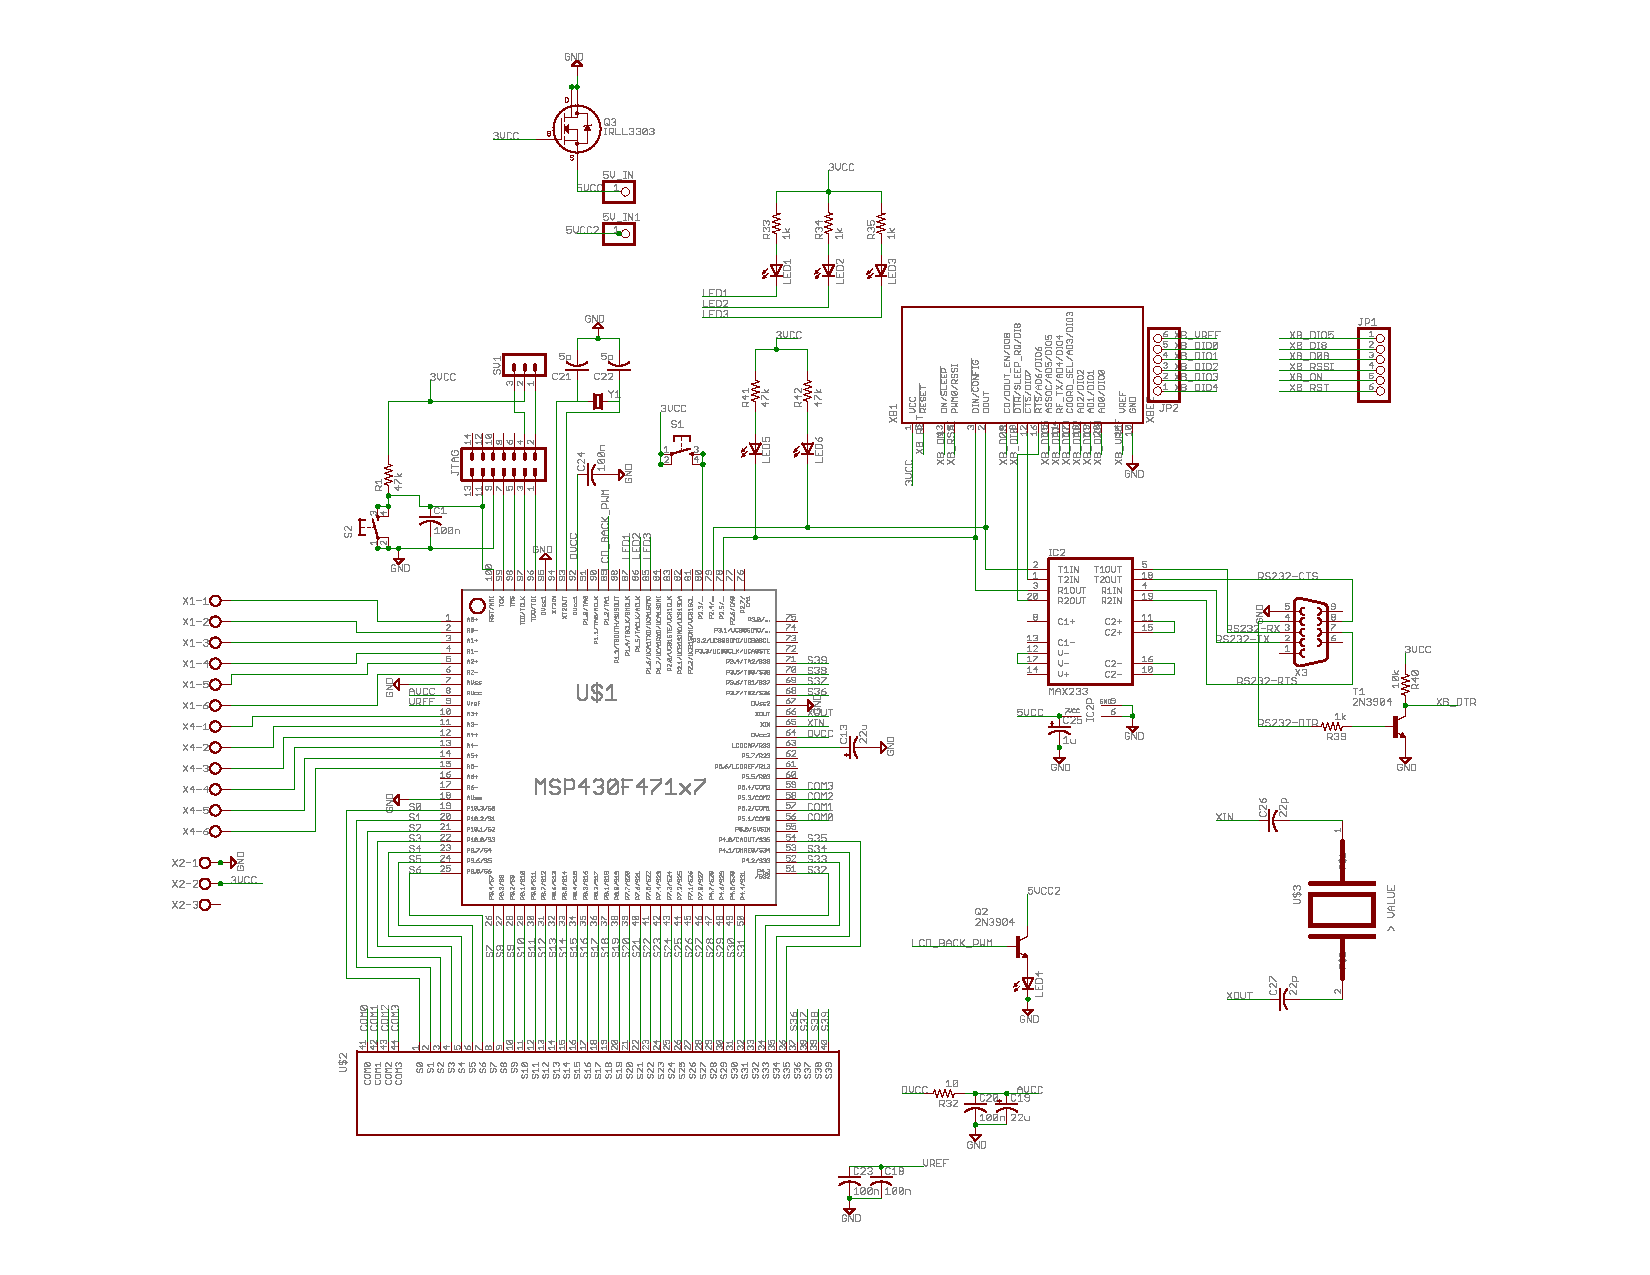
\includegraphics[height=5in, angle=90]{includes/E_Meter_Main_Schematic}
  \caption{E-Meter Main Board Schematic}
  \label{fig:e_meter_main_schematic_large}
\end{figure}

\begin{figure}[htbp]
  \centering
  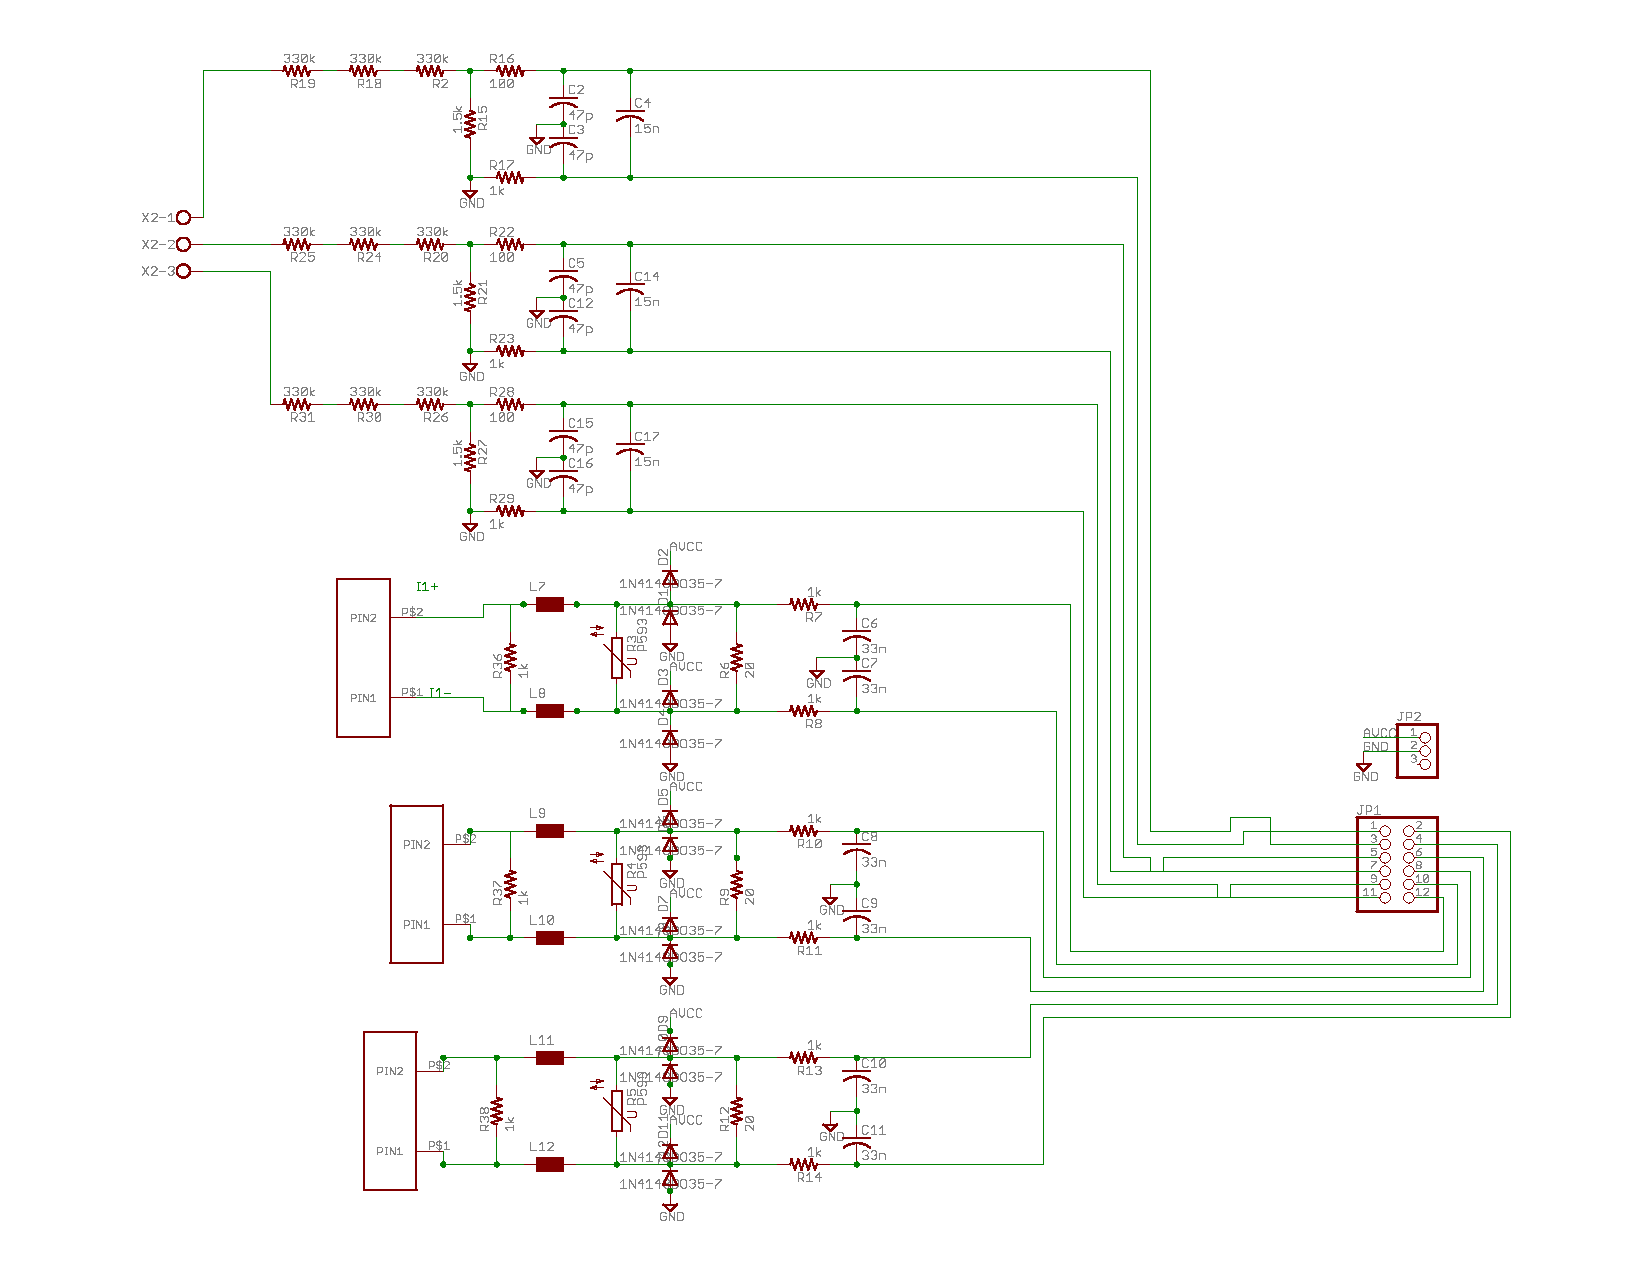
\includegraphics[height=5in, angle=90]{includes/e_meter_input_board_schem_large}
  \caption{E-Meter input board schematic.}
  \label{fig:e_meter_input_schematic_large}
\end{figure}
\clearpage

\subsection{E-Meter Printed Circuit Board}\label{sec:e_meter_pcb}
\begin{figure}[htbp]
  \centering
  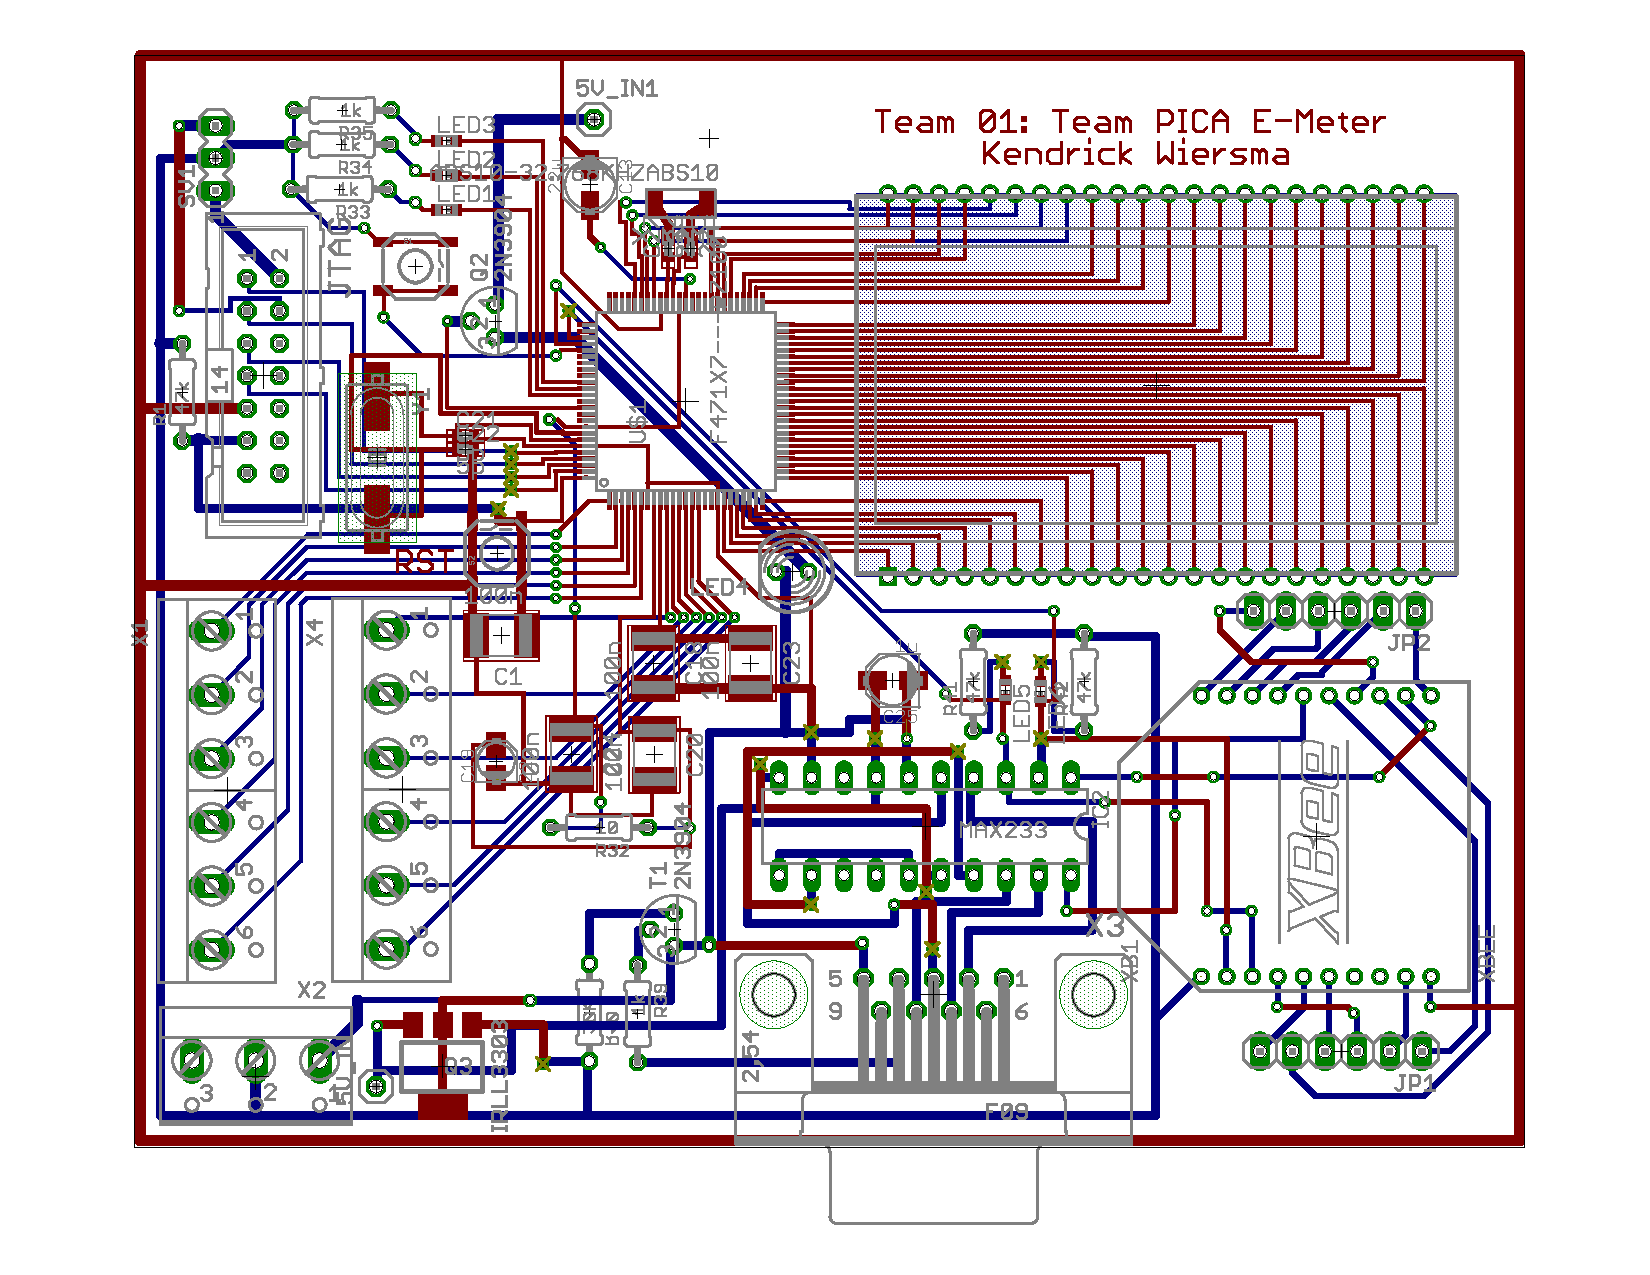
\includegraphics[width=5in, angle=90]{includes/e_meter_main_large}
  \caption{E-Meter main board.}
  \label{fig:e_meter_main_board_large}
\end{figure}
\begin{figure}[htbp]
  \centering
  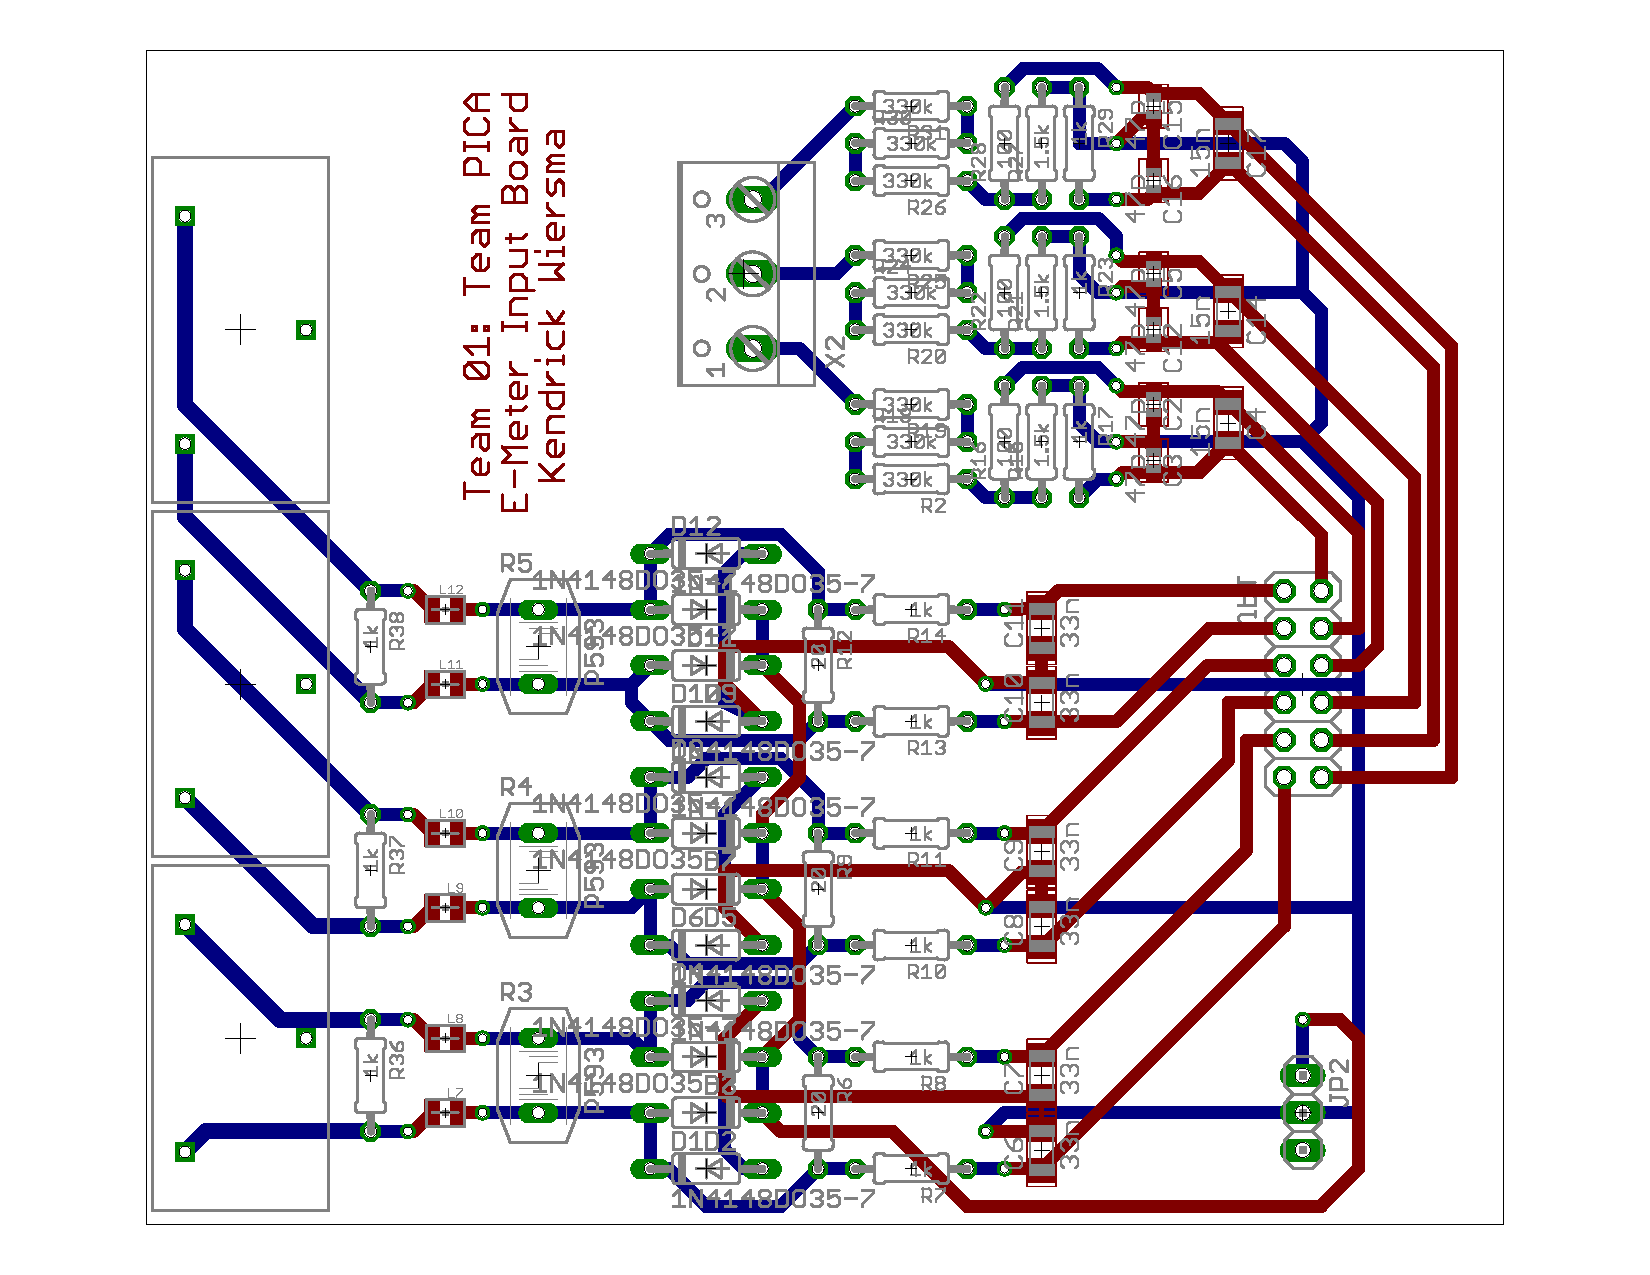
\includegraphics[height=5in, angle=90]{includes/e_meter_input_board_large}
  \caption{E-Meter input board.}
  \label{fig:e_meter_input_board_large}
\end{figure}
\clearpage

\subsection{E-Meter Code Listing}
\ccode{code/emeter_rc}{Final Measurement and Calculation Code}